\chapter{Teorema de Lax-Milgran}

Para dejar el puente libre, primero necesitamos ver nuestro funcional $L$ desde otro punto de vista. Para ello, vamos a ver una serie de definiciones y propiedades abstractas sobre los \textit{funcionales cuadráticos}, lo que nos va a permitir enunciar el teorema de Lax-Milgran, que nos dará la existencia de solución en esta última versión del modelo.

\begin{definition}\label{formabilineal}
Dados un cuerpo $K$ y un $K-$espacio vectorial $V$, una forma bilineal es una aplicación $\funcion{f}{V\times V}{K}$ que verifica:
\begin{enumerate}[(a)]
\item $f(u_1+u_2,v)=f(u_1,v)+f(u_2,v)$
\item $f(u, v_1+v_2)=f(u,v_1)+f(u,v_2)$
\item $f(au,v)=af(u,v)$
\item $f(u,av)=af(u,v)$
\end{enumerate}
para cualquier $a\in K$ y $u,v,u_1,u_2,v_1,v_2\in V$.

Una propiedad que necesitaremos es:
\[
f\left(\sum_ia_iu_i,\sum_jb_jv_h\right)=\sum_i\sum_ja_ib_jf(u_i,v_j)
\]

\end{definition}

\begin{definition}
Una forma bilineal $\funcion{f}{V\times V}{K}$ se dice simétrica si verifica:
\[
f(u,v)=f(v,u) \espacio \forall u,v\in V
\]
\end{definition}

\begin{definition}
Sea $H$ un espacio de Hilbert arbitrario, $\funcion{A}{H\times H}{\R}$ una forma bilineal, continua y simétrica y $\funcion{R}{H}{\R}$ una aplicación lineal y continua. Llamamos funcional cuadrático a la aplicación $\funcion{L}{H}{\R}$ dada por
\[
L(y)=\frac{1}{2}A(y,y)-R(y) \espacio\forall y\in H
\]
\end{definition}

\begin{definition}
Sea $\funcion{L}{H}{\R}$ una forma cuadrática. Diremos que es coerciva si existe una constante $\alpha\in\R^+$ tal que:
\[
A(u,u)\geq \alpha\norm{u}^2 \espacio \forall u\in H
\]
\end{definition}

\begin{prop}
Sea un espacio de Hilbert $H$ y $\funcion{L}{H}{\R}$ una forma cuadrátrica en ese espacio.
Entonces, la aplicación $\funcion{\norm{\cdot}_H}{H}{\R^+_0}$ definida por 
\[
\norm{u}_H=\sqrt{A(u,u)} \espacio \forall u\in H
\]
donde $\funcion{A}{H\times H}{\R}$ es la forma bilineal asociada a $L$, es una norma, y es equivalente a la norma natural de $H$.
\end{prop}
\begin{proof}
El hecho de que $\norm{\cdot}_H$ es una norma es sencillo de comprobar ya que $A$ define un producto escalar en $H$.

Sea $\funcion{\norm{\cdot}}{H}{\R}$ la norma de $H$. Necesitamos encontrar dos constante $c_1,c_2\in\R^+$ tal que 
\[
c_1\norm{u}\leq \norm{u}_H \leq c_2\norm{u}
\]
La constante $c_2$ la obtenemos por continuidad de la norma $\norm{\cdot}_H$ y la constante $c_1$ de la coercividad de $L$.

\end{proof}
A partir de ahora consideramos $\norm{\cdot}_H$ como nuestra norma por defecto en $H$.
\begin{prop}
Todo funcional cuadrático coercivo está acotado inferiormente.
\end{prop}
\begin{proof}
Sea $\funcion{L}{H}{\R}$ un funcional cuadrático, donde $\funcion{A}{H\times H}{\R}$ es su forma bilineal, continua y simétrica y $\funcion{R}{H}{\R}$ es su aplicación lineal y continua.
Vamos a ver que podemos acotar inferiormente la expresión de $L(y)$, con $y\in H$, por una función parabólica hacia arriba.

Como $R$ es continua, entonces $\norm{R(y)}\leq \norm{R}\norm{y} \Rightarrow -\norm{R(y)} \geq -\norm{R}\norm{y}$. Además, como $L$ es coerciva, existe cierta constante $C\in\R^+$ tal que $A(y,y)\geq C\norm{y}^2$. Combinando esas dos acotaciones, obtenemos:
\[
L(y)=\frac{1}{2}A(y,y)-R(y)\geq \frac{1}{2}C\norm{y}^2-\norm{R}\norm{y}
\]
Para ver con más claridad la parábola, hacemos el cambio $s=\norm{y}$, obteniendo una nueva función $P$ dependiente de las dos constantes $C$ y $\norm{R}$: $P(s)=\frac{1}{2}s^2-s\norm{R}$. Derivando e igualando a 0, obtenemos fácilmente que el mínimo de la parábola $P$ se alcanza en $s=\frac{\norm{R}}{C}$. Luego:
\[
L(y)\geq \frac{\norm{R}}{C} \espacio \forall y\in H 
\]

\end{proof}

\begin{theorem}[Lax-Milgran]
\label{laxmilgran}
Sea $\funcion{L}{H}{\R}$ un funcional cuadrático. Si $L$ es coercivo, entonces tiene mínimo absoluto en $H$.
\end{theorem}

\begin{prop}[condición de punto crítico]
\label{puntocritico}
Sea $\funcion{L}{H}{\R}$ un funcional cuadrático coercivo, $y\in H$. Entonces existe $y\in H$ verificando:
\[
A(\phi,y)-R(\phi)=0 \espacio \forall\phi\in\sobolev{}
\]

Además, el punto $y$ es el mínimo de $L$.
\end{prop}
\begin{proof}
Calculemos primero la expresión explícita de $g(s)$:
\[
g(s)=L(y+s\phi)=\frac{1}{2}A(y+s\phi,y+s\phi)-R(y+s\phi)
\]
Desarrollamos el primer término (usando la última propiedad en la definición \ref{formabilineal}):
\[
A(y+s\phi,y+s\phi)=A(y,y)+sA(y,\phi)+sA(\phi,y)+s^2A(\phi,\phi)=s^2A(\phi,\phi)+2sA(\phi,\phi)+A(y,y)
\]
Para el segundo término, usamos que $R$ es lineal:
\[
R(y+s\phi)=R(y)+sR(\phi)
\]
Quedándo:
\[
g(s)=\frac{1}{2}\left(s^2A(\phi,y)+2sA(\phi,\phi)+A(y,y)\right)-R(y)-sR(\phi)
\]
Derivando respecto de $s$:
\[
g(s)=sA(\phi,\phi)+A(\phi,y)-R(\phi) \Rightarrow g'(0)=A(\phi,y)-R(\phi)
\]
Luego nuestra condición de punto crítico es:
\[
A(\phi,y)-R(\phi)=0 \espacio \forall\phi\in\sobolev{}
\]

Para le existencia, simplemente tenemos que definir un producto escalar y usar el teorema de Riesz, como en los ejemplos anteriores. Sea $<<u,v>>=A(u,v)$ un producto escalar en $H$, por el teorema \ref{riesz-frechet}, existe $y\in H$ verificando:
\[
<<y,\phi>>=R(\phi) \espacio \forall \phi\in\\sobolev{}
\]

Para ver que es mínimo, tomamos $\funcion{g}{\R}{\R}$ definida por $g(s)=L(y+s(z-y))$. Notemos que $y+s(z-y)$ es la recta que una a $z$ con $y$. Tenemos que ver
\[
L(z)>L(y) \espacio \forall z\in H
\]
Que si nos fijamos, es equivalente a ver que
\[
g(1)>g(0)
\]
Que ya lo tenemos porque $s=0$ era el punto mínimo de la parábola.
\end{proof}

Una vez planteada toda la teoría necesaria, podemos volver a nuestro modelo del puente. Recordemos que nuestro funcional  $\funcion{L}{\sobolev{1}}{\R}$ venía dado por la expresión:
\[
L(y)=\frac{1}{2}\integral{a}{b}{y'(x)^2dx}+\frac{1}{2}\integral{a}{b}{K(x)y(x)^2dx}+\integral{a}{b}{q(x)y(x)dx}
\]
donde $q,K\in\lebesgue{\infty}$ y $K(x)\geq k_0 >0\ \casipordoquier$. La última condición la imponemos porque al dejar los extremos sueltos (lo hemos hecho al considerar como dominio de $L$ el espacio $\sobolev{1}$ en lugar de $\sobolevcero{1}$) necesitemos que el puente siga enganchado por las cuerdas.

Para poder usar la teoría desarrollada anteriormente, necesitamos ver que nuestro funcional es cuadrático. Definimos nuestra forma bilineal, continua y simétrica, y nuestra aplicación lineal y continua:
\[
A(u,v)=\integral{a}{b}{u'(x)v'(x)dx}+\integral{a}{b}{K(x)u(x)v(x)dx}, \; \espacio R(u)=-\integral{a}{b}{q(x)u(x)dx} \;\;\forall u,v\in\sobolev{1}
\]
Pero también necesitamos que $L$ sea coerciva. Usando la hipótesis sobre $K(x)$ es fácil de ver:
\[
A(u,u)=\integral{a}{b}{u'(x)^2dx}+\integral{a}{b}{K(x)u(x)^2dx}\geq\normasobolev{1}{u}^2+k_0\normasobolev{1}{u}^2\geq(1+k_0)\normasobolev{1}{u}^2
\]
Por lo tanto, sabemos que existe mínimo en $\sobolev{1}$. Además de saber que existe, queremos saber algo más sobre su expresión. Como hemos visto antes, los puntos críticos están caracterizados por la expresión:
\[
y\in\sobolev{1} \text{ punto critico } \Leftrightarrow A(y,\phi)=R(\phi) \espacio \forall \phi\in\sobolev{1}
\]
es decir,
\[
\integral{a}{b}{y'(x)\phi'(x)dx}+\integral{a}{b}{K(x)y(x)\phi(x)dx}=-\integral{a}{b}{q(x)\phi(x)dx} \espacio  \forall\phi\in\sobolev{1}
\]
Si en lugar de considerar $\phi$ en $\sobolev{1}$, la consideramos en $\soportecompacto$. Vemos que llamando $z=y'$ y agrupando los términos que tienen $\phi$, llegamos a:
\[
\integral{a}{b}{z(x)\phi'(x)dx}=-\integral{a}{b}{(K(x)y(x)+q(x))\phi(x)dx} \espacio  \forall\phi\in\sobolev{1}
\]

lo que significa que la derivada débil de $z$ es justamente $ky+q$. En particular z está en $\sobolev{1}$, porque todas las funciones que aparecen están en $\lebesgue{2}$. Luego debemos resolver la siguiente ecuación diferencial de orden 2 en $y$:
\[
y''(x)=K(x)y(x)+q(x) \espacio \forall x \in[a,b]
\]
Si imaginamos que $K$ y $q$ son continuas, esa ecuación tendría un gran número de soluciones. De hecho, el conjunto de soluciones sería un espacio biparamétrico (porque la solución depende de las condiciones iniciales sobre $y$ e $y'$). Tenemos que intentar limitarlas de alguna forma.

\begin{prop}\label{productoh1}
Sea $y\in\sobolev{1}$ (el representante continuo) y $\phi\in\mathcal{D}(\R)$, entonces $y\phi\in\sobolev{1}$.
\end{prop}
\begin{proof}
Para ver que $y\phi\in\sobolev{1}$, necesitamos encontrar su derivada débil. ¿Cuál es nuestro candidato a derivada débil? La derivada clásica, es decir, $z=y'\phi+y\phi'$. Para comprobarlo, tenemos que ver que para toda $\psi\in\soportecompacto$ se tiene:

\[
\integral{a}{b}{(y'(x)\phi(x)+y(x)\phi'(x))\psi(x)dx}+\integral{a}{b}{y(x)\phi(x)\psi'(x)dx}=0
\]
Reordenando los términos que tienen $y$ e $y'$, obtenemos:
\[
\integral{a}{b}{[\phi(x)\psi'(x)+\phi'(x)\psi(x)]y(x)dx}+\integral{a}{b}{[\phi(x)\psi(x)]y'(x)dx}=0
\]
Se cumple que si
$\phi \in \mathcal{D}(\mathbb{R}), \psi \in \mathcal{D}((a,b))$
entonce $\phi\psi \in \mathcal{D}((a,b))$ y
\[
  (\phi\psi)' = \phi'\psi + \phi\psi'
\]
Ahora por ser $y \in \mathcal{H}^1(a,b)$ y
$\hat\phi \in \mathcal{\mathbb{R}}$ tenemos que se cumple
\[
\integral{a}{b}{y'(x)\hat\phi(x)}+\integral{a}{b}{y(x)\hat\phi'(x)}=y(x)\hat\phi(x)\Big|^b_a
\]
una expresión general. Tomando $\hat\phi = \phi\psi$ tenemos que 

\[
\integral{a}{b}{y'(x)\hat\phi(x)}+\integral{a}{b}{y(x)\hat\phi'(x)}=y(x)\hat\phi(x)\Big|^b_a = 0
\]
ya que $\phi\psi(b) = \phi\psi(a) = 0$ y obtenemos así el resultado que buscabamos.
\end{proof}

Volviendo al problema original teníamos que

\begin{equation}
  \label{eq:probleminicial}
  \integral{a}{b}{y'(x)\phi(x)}+\integral{a}{b}{k(x)y(x)\phi(x)}=-\integral{a}{b}{q(x)\phi(x)}
\end{equation}


Considerando $\phi \in \mathcal{D}(\mathbb{R}), \phi \in \mathcal{H}^1$ y $z = y'$

obtenemos en la expresión anterior

\begin{equation}
  \label{eq:resparcial}
  \integral{a}{b}{z\phi'}=z\phi(x)\Big|^b_a - \integral{a}{b}{z'\phi}
\end{equation}

Como estabamos resolviendo el problema $y''=ky + q$ tenemos que se cumple

\[
\integral{a}{b}{z'\phi} = \integral{a}{b}{k(x)y(x)+q(x)\phi}
\]

y usando la igualdad que nos da \ref{eq:probleminicial} despejamos en
\ref{eq:resparcial} y obtenemos
\[
y'\phi\Big|^b_a = 0
\]

Si tomamos una $\phi$ como la siguiente

\centerline{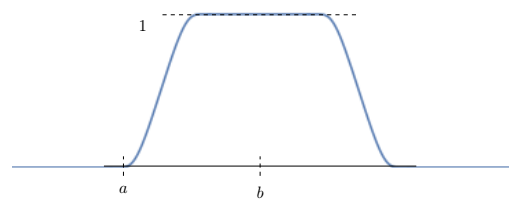
\includegraphics[scale=0.5]{img/caso1.png}} 

de la expresión $ 0 = y'\phi\Big|^b_a = y'(b)\phi(b)-y'(a)\phi(a)$
obtenemos $y'(b) = 0$. Tomando como $\phi$

\centerline{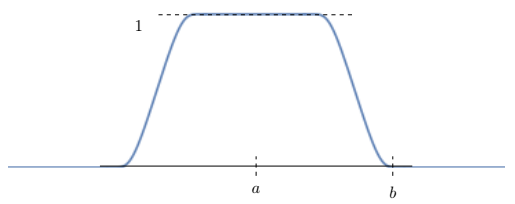
\includegraphics[scale=0.5]{img/caso2.png}} 

obtenemos $y'(a) = 0$. Dado que $z=y'\in \mathcal{H}^1$ entonces $y\in \mathcal{H}^2$ y
tomando el representante continuo obtenemos lo que se conoce como la condición de Neumann.

\section{La delta de Dirac y el espacio $H^{-1}$}

Ahora vamos a ver otro caso del modelo, donde colgamos una masa $m$ en un punto $\alpha\in(a,b)$ del puente. La energía de este objeto es $my(\alpha)$, luego la expresión de nuestro funcional $\funcion{L}{\sobolevcero{1}}{\R}$ es:
\[
L(y)=\frac{1}{2}\integral{a}{b}{y'(x)^2dx}+\frac{1}{2}\integral{a}{b}{q(x)y(x)^2dx}+my(\alpha)
\]
donde $y\in\sobolevcero{1}$, $q(x)\geq 0$ y  $q\in\lebesgue{\infty}$. La intuición nos dice que al colgar la masa $m$, se formará un pico en la cuerda, como muestra el siguiente dibujo:

\begin{center}
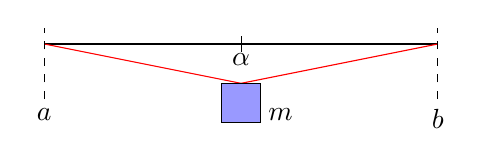
\begin{tikzpicture}
\draw (0,0) -- (5,0);
% parabola
\draw[scale=1,domain=0:2.5,smooth,variable=\x,red] plot ({\x}, {-0.2*\x});
\draw[scale=1,domain=2.5:5,smooth,variable=\x,red] plot ({\x}, {0.2*(\x-5)});

% etiquetas
\draw[dashed] (0,-0.7) -- (0,.2);
\draw (0,-0.7) node[anchor=north] {$a$};
\draw[dashed] (5,-.7) -- (5,.2);
\draw (5,-0.7) node[anchor=north] {$b$};
\draw (2.5,-0.1) -- (2.5,.1);
\draw (2.5,0) node[anchor=north] {$\alpha$};
\draw (3,-0.7) node[anchor=north] {$m$};

% masa
\fill[blue!40!white, draw=black] (2.25,-1) rectangle (2.75,-0.5);
\end{tikzpicture}
\end{center}
La forma bilineal $A$ es la misma que en el anterior modelo:
\[
A(y,y)=\frac{1}{2}\integral{a}{b}{y'(x)^2dx}+\frac{1}{2}\integral{a}{b}{q(x)y(x)^2dx}
\]
y como estamos en $\sobolevcero{1}$, $\integral{a}{b}{y'(x)^2dx}$ es una norma, luego $A$ es coercivo ya que restando el último término (que es positivo) obtenemos:
\[
A(y,y)\geq \frac{1}{2}\integral{a}{b}{y'(x)^2dx} = \frac{1}{2}\norm{u}^2
\] 
La aplicación lineal y continua $\funcion{R}{\sobolevcero{1}}{\R}$, viene dada por $R(y)=-my(\alpha)$, que tiene sentido al elegir el represante continuo porque $\sobolev{1}\subset \mathcal{C}(a,b)$. Por el teorema de Lax-Milgran (\ref{laxmilgran}) y la proposicion \ref{puntocritico}, existe $y\in\sobolevcero{1}$ de forma que
\[
A(y,\phi)=R(\phi) \espacio \forall \phi\in\sobolevcero{1}
\]
Lo que vamos a hacer ahora es calcular o ver qué condiciones verifica la función $y$. Usando la condición de punto crítico:
\begin{equation}
\label{formulageneral}
\integral{a}{b}{y'(x)\phi'(x)dx}+\integral{a}{b}{q(x)y(x)\phi(x)dx}=-m\phi(\alpha)
\end{equation}
Ahora hacemos una distinción de casos con $\phi$ perteneciendo a diferentes clases de Schwartz:
\begin{itemize}[-]
\item si $\phi\in\mathcal{D}(a,\alpha)$:
\[
\integral{a}{b}{y'(x)\phi'(x)dx}+\integral{a}{b}{q(x)y(x)\phi(x)dx}=-m\phi(\alpha)=0
\]
ya que $\alpha\notin(a,\alpha) \Rightarrow \phi(\alpha)=0$. Si denotamos $z=y'$, entonces $z\in\sobolev[a,\alpha]{1}\subset\mathcal{C}[a,\alpha]$ (porque la expresión anterior coincide con la definición de derivada débil para $z$).
\item si $\phi\in\mathcal{D}(\alpha,b)$, de igual forma conseguimos que $z\in\sobolevcero[\alpha,b]{1}\subset\mathcal{C}[\alpha,b]$. 
\end{itemize}
Fijaros que ese razonamiento no implica que $z\in\mathcal{C}[a,b]$, ya que el representante continuo usado en $[a,\alpha]$ y $[\alpha,b]$ son distintos. Lo que si implica es que $z\in\mathcal{C}\left([a,\alpha]\right)\cap \mathcal{C}\left([\alpha,b]\right)$ y existen los límites laterales de $\alpha$:
\[
z(\alpha^-)=\limite{x}{\alpha^-}{z(x)} \espacio z(\alpha^+)=\limite{x}{\alpha^+}{z(x)}
\]
Además sabemos que $z'=qy \;\; a.e \; x \in(a,\alpha)\cup(\alpha,b)$. Si volvemos a la fórmula general \eqref{formulageneral}:
\begin{equation}
\label{formulageneral2}
\integral{a}{b}{z(x)\phi'(x)dx}+\integral{a}{b}{q(x)y(x)\phi(x)dx}=-m\phi(\alpha) \espacio \forall\phi\in\sobolevcero{1}
\end{equation}
Ahora queremos desarrollar esa expresión. Tomamos $\phi\in\soportecompacto$, como $z$ no es continua en $\alpha$, la integral del primer término hay que escribirla en dos partes:
\[
\integral{a}{b}{z(x)\phi'(x)dx}=\integral{a}{\alpha}{z(x)\phi'(x)dx}+\integral{\alpha}{b}{z(x)\phi'(x)dx}
\]
Aplicamos derivación por partes a cada término:
\[
\integral{a}{\alpha}{z(x)\phi'(x)dx}=z(x)\phi(x)\Big|_a^\alpha-\integral{a}{\alpha}{z'(x)\phi(x)dx}=z(\alpha^-)\phi(\alpha)-\integral{a}{\alpha}{z'(x)\phi(x)dx}
\]
\[
\integral{\alpha}{b}{z(x)\phi'(x)dx}=z(x)\phi(x)\Big|_\alpha^b-\integral{\alpha}{b}{z'(x)\phi(x)dx}=-z(\alpha^+)\phi(\alpha)-\integral{\alpha}{b}{z'(x)\phi(x)dx}
\]
Combinando los resultados y sustituyendo en \eqref{formulageneral2}:
\[
z(\alpha^-)\phi(\alpha)-z(\alpha^+)\phi(\alpha)-\integral{a}{b}{z'(x)\phi(x)dx}=-\integral{a}{b}{z'(x)\phi(x)dx}-m\phi(\alpha)
\]
Cancelando ámbos términos:
\[
\left(z(\alpha^-)-z(\alpha^+)\right)\phi(\alpha)=-m\phi(\alpha)
\]
Como la función de Schwartz escogida es arbitraria, podemos suponer que vale 1 en $\alpha$. Usando eso y que $z=y'$:
\[
y'(\alpha^-)-y'(\alpha^+)=-m \Rightarrow y'(\alpha^+)-y'(\alpha^-)=m  
\]
Es decir, el cambio de pendiente que se da entre $\alpha^-$ y $\alpha^+$ es igual a $m$, el peso de la masa.

\section{Sturm-Liouville: caso 1}\label{slc1}

Vamos a generalizar el caso anterior para obtener una ecuación diferencial con varias condiciones. Sea $\funcion{L}{\sobolev{1}}{\R}$ el funcional dado por:
\[
L(y)=\frac{1}{2}\integral{a}{b}{y'(x)^2dx}+\frac{1}{2}\integral{a}{b}{q(x)y(x)^2dx}-R(y)
\]
con $q\in\lebesgue{\infty}$, $0<q_0\leq q(x)\leq q_1 \; \casipordoquier$. 

De donde podemos definir la siguiente forma cuadrática: 
\[
A(y,\phi)=\integral{a}{b}{y'(x)\phi'(x)dx}+\integral{a}{b}{q(x)y(x)^2\phi(x)dx}
\]
Una vez más, la teoría de Lax-Milgran nos dice que existe $y$ en $\sobolev{1}$ cumpliendo $A(y,\phi)=R(\phi)$, es decir, $ \forall R\in \sobolev{-1}=\left(\sobolev{1}\right)^*$:
\begin{equation}
\label{condicion1}
\integral{a}{b}{y'(x)\phi'(x)dx}+\integral{a}{b}{q(x)y(x)\phi(x)dx}=R(\phi) \;\; \forall \phi\in\sobolev{1}
\end{equation}

Una vez planteado el problema y visto que tiene solución, tenemos que intentar determinar $y$ mediante alguna ecuación diferencial. Como vamos a determinar $y$ mediante una ecuación diferencial, necesitamos buscar condiciones de regularidad sobre ella porque la teoría de ecuaciones diferenciales nos dice que hay solución siempre que los elementos de la ecuación sean continuos. Nótese que, por ahora, solo sabemos que $y\in\continuas$ e $y'\in\lebesgue{2}$.
   
Ahora vamos a empezar con el primer caso. Partimos de la condición \eqref{condicion1} y recordamos que tenemos la cadena de espacios:
\[
\lebesgue{2} = \sobolev{0} \subset \sobolev{-1}
\]

Donde la indentificación $\sobolev{0}\longhookrightarrow\sobolev{-1}$ viene dada por la aplicación
\[
\begin{array}{ll}
R: & \lebesgue{2} \longrightarrow \sobolev{-1} \\
  &\;\;\; r \;\;\; \;\;\;\; \longmapsto    \funcion{R_r}{\sobolev{2}}{\R} \\
  & \hspace*{3cm} y \mapsto R_r(y)=\integral{a}{b}{r(x)y(x)dx} 
\end{array}
\]

Nótese ahora que si denotamos $z=y'$, la ecuación \eqref{condicion1} nos dice que se verifica:
\begin{equation}
\label{condicion2}
\integral{a}{b}{z(x)\phi'(x)dx}+\integral{a}{b}{q(x)y(x)\phi(x)dx}=\integral{a}{b}{r(x)\phi(x)dx}
\end{equation}
Y agrupando:
\[
\integral{a}{b}{z(x)\phi'(x)dx}+\integral{a}{b}{\left(q(x)y(x)-r(x)\right)\phi(x)dx}=0
\]
Luego $z$ tiene derivada débil y coincide con $z'=qy-r$. Como $z'=y''$, nos queda la EDO:
\[
y''-qy=-r \Rightarrow -y''+qy=r
\]
Ahora, como $z$ tiene derivada débil, puedo tomar su representante continuo $\bar{z}\in\continuas$, es decir, podemos suponer directamente que $z\in\continuas$. Pero claro, como $z=y'$, entonces $y'\in\continuas$, lo que implica que $y\in\continuas[1]$. En particular, tenemos definido cuanto vale $y'(a)$ e $y'(b)$ (antes no lo teníamos porque solo sabíamos que $y\in\lebesgue{2}$). Luego la ecuación $-y''+qy=r$ se verifica en $\sobolev{2}$ (porque $z\in\sobolev{1}$, luego $y\in\sobolev{2}$).

Se puede comprobar fácilmente que si $r,q\in\continuas$ entonces $y\in\continuas[2]$, debido a que en ese caso, $y''$ sería continua (se expresaría como diferencia de continuas y producto de continuas).

Como la expresión \eqref{condicion2} es válida para toda $\phi\in\sobolev{1}$, podemos tomar una $\phi\in\mathcal{D}(\R)$ y como $z\in\sobolev{2}$, la proposición \ref{productoh1} nos dice que $z\phi\in\sobolev{1}$ y $\left(z\phi\right)'=z\phi'+z'\phi$. Usando integración por partes en el primer término:
\[
\integral{a}{b}{z(x)\phi'(x)dx}=z(x)\phi(x)\Big|_a^b-\integral{a}{b}{z'(x)\phi(x)dx}=
\]
\[
=z(b)\phi(b)-z(a)\phi(a)-\integral{a}{b}{(q(x)y(x)-r(x))\phi'(x)dx}
\]
Sustituyendo ahora lo obtenido en la expresión \eqref{condicion2} y simplificando, llegamos a:
\[
z(b)\phi(b)-z(a)\phi(a)=0 \espacio \forall \phi \in\mathcal{D}(\R)
\]
Si ahora tomamos una función $\phi$ de la siguiente forma:

\centerline{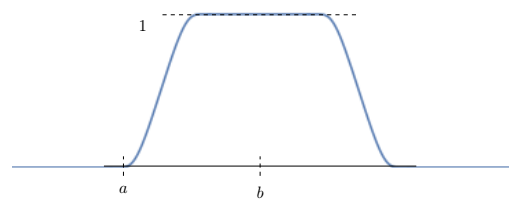
\includegraphics[scale=0.5]{img/caso1.png}} 

Entonces $\phi(a)=0$ y $\phi(b)=1$, de donde queda que $z(b)=0$. Tomando otra $\phi$ de esta forma
\centerline{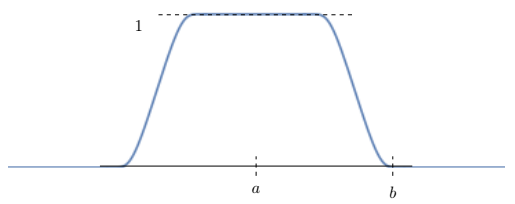
\includegraphics[scale=0.5]{img/caso2.png}} 

obtenemos que $z(a)=0$. Es decir, $y'(a)=y'(b)=0$.

\section{Sturm-Liouville: caso 2}

Para el siguiente caso tenemos que definir primero la \textit{delta de Dirac}.

\medskip

\begin{definition}
Dado $\alpha\in(a,b)$, definimos la función $\funcion{\delta_\alpha}{\sobolev{-1}}{\R}$
\[
\delta_\alpha(y)=y(\alpha), \espacio \delta_\alpha\in\sobolev{1}, \;\; \delta_\alpha\notin\sobolev{0}
\]
A $\delta_\alpha$ la llamaremos \textit{delta de Dirac}.
\end{definition}
\begin{remark}
Nótese que esta función simplemente es otra forma de denotar la evaluación en $\alpha$, que usamos para indicar en qué punto $\alpha$, de una cuerda $y$, colgamos una masa $c$. 
\end{remark}

Ahora pasamos al siguiente caso, donde suponemos que $R(\phi)=c\delta_\alpha(\phi)=c\phi(\alpha) \espacio \forall \phi\in\sobolev{1}\subset\continuas$, con $a<\alpha<b$. Con esta nueva $R$, vemos otra vez la ecuación \ref{condicion1} con $z=y'$:
\[
\integral{a}{b}{z(x)\phi'(x)dx}+\integral{a}{b}{q(x)y(x)\phi(x)dx}=c\phi(\alpha)
\]
donde solo sabemos que $z\in\lebesgue{2}$ e $y\in\sobolev{1}$ y $z$ no tiene por qué tener derivada débil ya que la expresión anterior no coincide con la de la definición. 

Si ahora considero el intervalo $(a,\alpha)$ y tomo $\phi\in\mathcal{D}(a,\alpha)$, tenemos que $\phi(\alpha)=0$ y
\[
\integral{a}{b}{z(x)\phi'(x)dx}+\integral{a}{b}{q(x)y(x)dx}=0
\]
Luego $z\in\sobolev[a,\alpha]{1}$, que tiene un representante continuo $z_1\in\mathcal{C}[a,\alpha]$. De forma análoga, obtenemos $z_2\in\mathcal{C}[\alpha,b]$. Si definimos $z'$ como la unión de $z_1'$ y $z_2'$:
\[
z'(x)= \left\{
\begin{array}{cc}
z_1'(x) & x\in(a,\alpha) \\
z_2'(x) & x\in(\alpha,b)
\end{array}
\right.
\]
¿y qué pasa con $z'(\alpha)$? No pasa nada, porque $\{\alpha\}$ tiene medida nula asi que no hace falta definirla en ese punto. Además, $z'\in L^2(a,\alpha)$ y $z'\in L^2(\alpha,b)$, luego $z'\in\lebesgue{2}$ por la misma razón. 

Como $z'$ no es la derivada débil de $z$ en $(a,b)$, solo podemos decir que
\[
\integral{a}{b}{z'(x)\phi(x)dx}+\integral{a}{b}{z(x)\phi'(x)dx}=0 \espacio \forall \phi\in\mathcal{D}(a,\alpha) \text{ ó } \forall \phi\in\mathcal{D}(\alpha,b)
\]
Y en ese caso, $z'(x)=-q(x)y(x) \;\; \casipordoquier$. 

Como vemos, este es el origen de la cuestión, tenemos una función $z'$, que sabemos que es una derivada, pero es una derivada \textit{extraña}, ya que es débil en $(a,\alpha)$ y $(\alpha,b)$, coincide en casi todo punto con $-q(x)y(x)$, pero no es una derivada débil en $(a,b)$. 

En principio, no sabemos si $z$ es continua, lo único que sabemos es que $z_1$ y $z_2$ sí lo son, y se cumple:
\[
\begin{array}{cc}
z(x)=z_1(x) & \text{ a.e } x\in(a,\alpha) \\
z(x)=z_2(x) & \text{ a.e } x\in(\alpha,b)
\end{array}
\]
Usando esa propiedad, podemos definir otra función, $z_3$, como sigue:
\[
z_3(x)=\left\{
\begin{array}{cc}
z_1(x) & x\in[a,\alpha) \\
z_2(x) & x\in(\alpha,b]
\end{array}
\right.
\]
Fijaros que $z_3$, por el carácter local de la continuidad, es continua en $(a,\alpha)$ y $(\alpha,b)$. De hecho, es continua en $a$ y $b$ también porque coincide con $z$ en ese entorno. Además, se verifica:
\[
\begin{array}{c}
\limite{x}{\alpha^-}{z_3(x)}=\limite{x}{\alpha^-}{z_1(x)}=z_1(\alpha)\\
\limite{x}{\alpha^+}{z_3(x)}=\limite{x}{\alpha^+}{z_2(x)}=z_2(\alpha)
\end{array}
\]
Es decir, $z_3$ no es continua en $[a,b]$, pero sí tienes límites laterales. Además, la discontinuidad que presenta en $\alpha$ es evitable (ojo, que no es seguro que siempre la tenga). De ahora en adelante, vamos a denotar simplemente por $z$ a $z_3$, ya que no tiene mucho sentido arrastrar ambas notaciones. 

Ahora vamos a razonar con $z_1$, que es una solución en $(a,\alpha)$, luego por la condición de punto crítico, tenemos que:
\[
\integral{a}{b}{z_1(x)\phi'(x)dx}+\integral{a}{b}{q(x)y(x)\phi(x)dx}=0 \espacio \forall\phi\in\mathcal{D}(a,\alpha)
\]
Si consideramos ahora $\phi$ sobre $\mathcal{D}(\R)$ en lugar de sobre $\mathcal{D}(a,\alpha)$, tenemos que:
\[
\integral{a}{\alpha}{z_1(x)\phi'(x)dx}+\integral{a}{\alpha}{q(x)y(x)\phi(x)dx}=0
\] 
Aplicando integración por partes al primer término:
\[
\integral{a}{\alpha}{z_1(x)\phi'(x)dx}=z_1(x)\phi(x)\Big|_a^\alpha-\integral{a}{\alpha}{q(x)y(x)\phi(x)dx}
\]
Cogiendo la $\phi$ de forma que $\phi(a)=1$ y $\phi(x)=0\quad\forall x\geq\alpha$, y sustituyendo en la expresión anterior:
\[
-z_1(a)\phi(a)-\integral{a}{\alpha}{q(x)y(x)\phi(x)dx}+\integral{a}{\alpha}{q(x)y(x)\phi(x)dx}=0 \Rightarrow -z_1(a)\phi(a)=0
\]
Es decir, $z_1(a)=0$. De forma análoga, se prueba que $z_2(b)=0$. Eso implica que $y'(a)=y'(b)=0$, luego: 
\[
\left.
\begin{array}{cc}
y\in\sobolev[a,\alpha]{2}\\
y\in\sobolev[\alpha,b]{2}
\end{array}
\right\} \Rightarrow
\left.
\begin{array}{cc}
y\in\mathcal{C}^1[a,\alpha]\\
y\in\mathcal{C}^1[\alpha,b]
\end{array}
\right\}
\]
En conclusión, hemos llegado a la ecuación diferencial
\[
-y''(x)+q(x)y(x)=0
\]
que sólo se cumple en $(a,\alpha)$ y $(\alpha,b)$. Quedaría ver qué pasa en el extremo, aunque más o menos se ve que simplemente no van a coincidir las derivadas laterales: $y'(\alpha^+)-y'(\alpha^-)=-c$

\section{Sturm-Liouville: caso 3}\label{slc3}

Podemos combinar los dos casos anteriores, para resolver el caso donde $R$ vene dado por:
\[
R(x)=r(x)+\sum_{i=1}^nc_i\delta_{\alpha_i} \espacio a<\alpha_1<\cdots<\alpha_n<b
\]
donde $y\in\sobolev{1}$, $y\in\mathcal{H}^2\left((a,\alpha_1)\cup\dots\cup(\alpha_n,b)\right)$, $y\in\mathcal{C}^1\left((a,\alpha_1)\cup\dots\cup(\alpha_n,b)\right)$, y por supuesto $y\in\mathcal{C}[a,b]$. La ecuación diferencial de este caso es la misma que en los dos anteriores:
\[
-y''(x)+p(x)y(x)=r(x)
\]
Esta igualdad es una igualdad puntual y la $y''$ es derivada débil en
cada uno de los trocitos. La \textit{condición de contorno} también se
verifica: $y'(a)=y'(b)=0$ y $y'(\alpha^+_i)-y'(\alpha^-_i)=-c_i$.

\section{Sturm-Liouville: caso 4}

En este caso, en lugar de minimizar en $\sobolev{1}$, podemos hacerlo en $\sobolevcero{1}$. La única diferencia es que la concición $y'(a)=y'(b)=0$ se sustituye por
\[
y(a)=y(b)=0
\]
Además, basta tomar $0\leq q(x)\leq q_1$. En este caso también podemos suponer que 
\[
R(x)=r(x)+\sum_{i=1}^nc_i\delta_{\alpha_i} \espacio a<\alpha_1<\cdots<\alpha_n<b
\]
verificándose casi lo mismo que en el caso anterior: $y\in\sobolev{1}$, $y\in\mathcal{H}^2\left((a,\alpha_1)\cup\dots
\cup(\alpha_n,b)\right)$, $y\in\mathcal{C}^1\left((a,\alpha_1)\cup\dots\cup(\alpha_n,b)\right)$, $y\in\mathcal{C}[a,b]$ y
$y'(\alpha^+_i)-y'(\alpha^-_i)=-c_i$ pero $y(a)=y(b)=0$.

\section{Sturm-Liouville: caso 5}\label{slc5}

En este caso vamos a considerar la densidad del puente, por lo que nuestro funcional cambia un poco:
\[
L(y)=\frac{1}{2}\integral{a}{b}{p(x)y'(x)^2dx}+\frac{1}{2}\integral{a}{b}{q(x)y(x)^2dx}-R(y)
\]
Con las condiciones: $0<p_0\leq p(x) \leq p_1$, $0<q_0\leq q(x) \leq q_1$.
Con este planteamiento, la ecuación que se verifica es:
\[
\integral{a}{b}{p(x)y'(x)\phi'(x)dx}+\integral{a}{b}{q(x)y(x)\phi(x)dx}=R(\phi) \espacio \forall \phi\in\sobolev{1}
\]
con $y\in\sobolev{1}$, $y\in\mathcal{C}[a,b]$. Si tomo $z(x)=p(x)y'(x)$, ¿cuáles son las condiciones de regularidad?
\begin{enumerate}[(a)]
\item Si $R(x)=r(x)$, entonces $z\in\sobolev{1}$ y $z\in\continuas$. Además:
\[
-(p(x)y'(x))'+q(x)y(x)=r(x)
\]
Y $z(a)=z(b)=0$.
\item Si cambiamos $\sobolev{1}$ por $\sobolevcero{1}$, la condición $z(a)=z(b)=0$ la tenemos que cambiar por $y(a)=y(b)=0$. Y en este caso, basta con que se cumpla $0\leq q(x)\leq q_1$.
\item Si $R(x)=r(x)+\sum_{i=1}^nc_i\delta_{\alpha_i} \espacio a<\alpha_1<\cdots<\alpha_n<b$ e $y\in\sobolev{}$. Luego $z\in\sobolev[a,\alpha_1]{1}$, $\cdots$, $z\in\sobolev[\alpha_n,b]{1}$, e igual con las continuas: $z\in\mathcal{C}[a,\alpha_1]$, $\cdots$, $z\in\mathcal{C}[\alpha_n,b]$. La ecuación que se verifica es:
\[
(p(x)y'(x))'+q(x)y(x)=r(x)
\]
Con la condición de contorno $z(a)=z(b)=0$ (si $\sobolev{}$) ó $y(a)=y(b)=0$ (si $\sobolevcero{1}$). Las condiciones en las derivadas laterales son:
\[
z(\alpha^+_i)-z(\alpha_i^-)=-c_i
\]
\end{enumerate}

\section{Casos regulares}

Procedemos ahora a replantear los problemas anteriores bajo la
hípotesis de que $R=r(x)$ con $r\in\continuas$, $q\in\continuas$ con
\[
\begin{array}{rr}
0<q_0\leq q(x)\leq q_1 & \text{ si } \sobolev{1}\\
0\leq q(x) \leq q_1    & \text{ si } \sobolevcero{1}
\end{array}
\]
\subsection{Sturm-Liouville: caso regular (1)}

Trabajamos en el mismo caso que \eqref{slc1} con esta nuevas
hipótesis. Tenemos $y\in\sobolev{1}$ y nuestro funcional (sin considerar la densidad del puente)
es:
\[
L(y)=\frac{1}{2}\integral{a}{b}{y'(x)^2dx}+\frac{1}{2}\integral{a}{b}{q(x)y(x)^2dx}-R(y)
\]

De aquí obtenemos que $y\in\sobolev{2}$ de donde tendríamos que se verificaría la condición
\[
 -y'' + q(x)y(x) = r(x)
\]

que al igual que nos pasaba antes es una igualdad que se da en sentido
puntual. Despejando de esta ecuación, ya que $y\in\continuas$,
obtenemos que $y''\in\continuas$ y por tanto
$y\in\continuas[2]$. Tenemos ahora las herramientas para resolver el
problema con la formula de variación de constantes y las condiciones
iniciales.

\subsection{Sturm-Liouville: caso regular (2)}

Procedemos como en el caso \eqref{slc3}, es decir, partimos de :
\[
R(\phi)=r(x)+\sum_{i=1}^nc_i\delta_{\alpha_i} \espacio a<\alpha_1<\cdots<\alpha_n<b
\]

y con $y\in\mathcal{H}^2(\alpha_i,\alpha_{i+1})$ donde en cada intervalo tenemos la ecuación diferencial, en sentido debil:
\[
 -y'' + q(x)y(x) = r(x)
\]

esto quiere decir que en cada intervalo
$y\in\mathcal{C}^2[\alpha_i,\alpha_{i+1}]$. Ahora se cumplen unas
condiciones que son propia de la $y$ y no de un representante continuo:

\[
\begin{array}{rr}
y'(a) = y'(b) = 0 & \text{ si } \sobolev{1}\\
y(a) = y(b) = 0    & \text{ si } \sobolevcero{1}
\end{array}
\]

y la condición sobre la delta de dirac es que
$y'(\alpha_i^+) - y'(\alpha_i^-) = c_i$ por lo que si $c_i \neq 0$ se
tiene que $y\notin\mathcal{C}^1[a,b]$


\subsection{Sturm-Liouville: caso regular (3)}
Como en el caso \eqref{slc5} procedemos a añadir un peso con las
hipótesis que estamos manejando.

\[
L(y)=\frac{1}{2}\integral{a}{b}{p(x)y'(x)^2dx}+\frac{1}{2}\integral{a}{b}{q(x)y(x)^2dx}-R(y)
\]

pero voy a imponer que $p\in\continuas[1]$ y
$0 < p_o \leq p(x) \leq p_1$. Tendríamos así que
$p(x)y'(x)\in\sobolev{1}$ y usando el resultado \eqref{productoh1}
bajo unas condicion más fuertes donde $\phi\in\continuas$ podemos ver
que

\[
 y'(x) = \frac{1}{p(x)}p(x)y'(x) \in \sobolev{1} \label{regular3prod}
\]

y en particular $y\in\sobolev{2}$. Sobre la cuestión de la derivada
debil

\[
-(p(x)y'(x))' + q(x)y(x)=r(x)
\]

y derivando obtenemos que

\[
-p(x)'y'(x)  - p(x)'y''(x) + q(x)y(x) = r(x)
\]

y despejando $y''$ obtenemos que $y\in\continuas[2]$. Ahora adaptamos
la condición de contorno. En el caso anterior se verificaba
$z(a) = z(b) = 0$ con $z(x) = p(x)y'(x) \in \continuas$ luego
\[
  p(a)y'(a) = 0 \text{ y } p(b)y'(b) = 0 \implies y'(a) = y'(b) = 0
\]

en el caso de $\sobolev{1}$ y en el caso de $\sobolevcero{1}$

\[
  y(a) = 0 \text{ y } y(b) = 0
\]

\textbf{(AQUI EMPIEZA LA CLASE DEL 14 DE ABRIL)}

\section{Problema de Sturm-Liouville regular}

En esta sección vamos a cambiar la notación, lo que antes represantábamos por $y$ lo vamos a denotar por $u$. Con esta notación, nuestro funcional quedaría:
\begin{equation}\label{ff}
L(u)=\frac{1}{2}\integral{a}{b}{p(x)u'(x)^2dx}+\frac{1}{2}\integral{a}{b}{q(x)u(x)^2dx}-R(u)
\end{equation}

Tenemos la ecuación (de los casos anteriores):
\begin{equation}\label{ec}
-(p(x)u'(x))'+q(x)u(x)=r(x) \espacio \forall x\in[a,b]
\end{equation}
con las siguientes condiciones de contorno:
\begin{equation}\label{eq:ca}
\alpha_au(a)+\beta_au'(a)=\gamma_a \tag{$c_a$}
\end{equation}
\begin{equation}\label{eq:cb}
\alpha_bu(b)+\beta_bu'(b)=\gamma_b \tag{$c_b$}
\end{equation}
donde $p\in\continuas[1]$, lo que nos dice que el primer término de \eqref{ec} se puede desarrollar para obtener una EDO (recordemos, que necesitamos que todas los elementos sean continuos para poder aplicar la teoría que sabemos de ecuaciones diferenciales). Además, $p(x)>0$ si $x\in[a,b]$ (para que podemos hacer cocientes luego). $q,r\in\continuas$ y $(\alpha_a,\beta_a)\neq(0,0)$, $(\alpha_b,\beta_b)\neq(0,0)$.

A la ecuación anterior y al conjunto de condiciones de contorno anteriores, es lo que vamos a denominar el \textit{problema de Sturm-Liouville regular}. Recordemos que tenemos varios casos ya conocidos y que hemos resuelto. Reescribámoslos con esta nueva notación del problema:
\begin{enumerate}[(a)]
\item (Dirichlet) $(\alpha_a,\beta_a)=(1,0)=(\alpha_b,\beta_b)$, $\gamma_a=\gamma_b=0$. Además había que imponer $q(x)\geq 0$ $x\in[a,b]$. En estas condiciones, existe una única solución del problema.

Para comprobarlo, lo único que tenemos que hacer es minimizar en $\sobolevcero{1}$ el funcional dado por \eqref{ff} con $R(u)=\integral{a}{b}{r(x)u(x)dx}$. Al resolverlo, obtenemos $u\in\continuas[2]$.

La solución de este caso, es la misma que la del siguiente problema:
\[
\min\left\{L(u):\; u\in\continuas[2],\; u(a)=u(b)=0\right\}
\]
A ese espacio se le suele llamar $C_0^2[a,b]$. El problema es que ese espacio es de Banach pero no es reflexivo, luego no puede ser de Hilbert, es decir, nada de la teoría que desarrollamos anteriormente vale para este espacio.

\item (Neumann) $(\alpha_a,\beta_a)=(0,1)=(\alpha_b,\beta_b)$, $\gamma_a=\gamma_b=0$, $q(x)>0$ $x\in[a,b].$ La condición sobre $q$ la ponemos porque una función continua en un compacto alcanza el mínimo, luego si imponemos que sea positiva en todo el intervalo, ese mínimo también será positivo. En estas condiciones, existe una única solución en $\sobolev{1}$. Igual que antes, esta solución coincide con la solución de:
\[
\min\left\{L(u):\; u\in\continuas[2]\right\}
\]
De hecho, también se da que es:
\[
\min\left\{L(u):\; u\in\continuas[2],\; u'(a)=u'(b)=0\right\}
\]
\end{enumerate}

\begin{remark}
Sea $A\in\mathcal{M}_{n\times n}(\R)$, $x,b\in\R^n$ y queremos resolver el sistema $Ax=b$. Si $Ax=0$  tiene una única solución, entonces el sistema completo también tiene una única solución.
\end{remark}

Al principio de esta sección, planteamos el \textit{problema de Sturm-Liouville regular}, si se da el caso de que $r(x)=0$ para $x\in[a,b]$ y $\gamma_a=\gamma_b=0$, es decir, tendríamos la ecuación
\[
-(p(x)u'(x))'+q(x)u(x)=0 \espacio \forall x\in[a,b]
\]
con las condiciones de contorno:
\begin{equation}\label{eq:ha}
\alpha_au(a)+\beta_au'(a)=0 \tag{$h_a$}
\end{equation}
\begin{equation}\label{eq:hb}
\alpha_bu(b)+\beta_bu'(b)=0 \tag{$h_b$}
\end{equation}
entonces lo denotaremos por \textit{problema de Sturm-Liouville homogéneo}. 
\begin{remark}
Por abreviar en la notación, de ahora en adelante usaremos las siguientes convenciones para diferenciar entre el problema homogéneo y el completo (o regular):
\begin{equation}\label{eq:psl}
-(p(x)u'(x))'+q(x)u(x)=r(x) \espacio \forall x\in[a,b]\tag{PSL}
\end{equation}
\begin{equation}\label{eq:pslh}
-(p(x)u'(x))'+q(x)u(x)=0 \espacio \forall x\in[a,b]\tag{PSLH}
\end{equation}
Además, cuando digamos que una función verifica $(PSL)+c_a$, estaremos diciendo que las condiciones iniciales de la solución cumplen $c_a$ y la ecuación diferencial dada por $(PSL)$. Igual con $(PSLH)$, $c_b$, $h_a$ y $h_b$.
\end{remark}

Veamos ahora un lema que nos ayudará en la demostración del siguiente teorema.

\begin{lemma}
Las soluciones de la ecuación diferencial (PSL) que verifican la condición $c_a$ son de la forma:
\[
u_1(t)+\lambda u_2(t)
\]
donde $\lambda\in\R$, $u_1$ es una solución particular de $(PSL)$ junto con la condición $c_a$, y $u_2$ es una solución no trivial de $(PSLH)$ junto con la condición $h_a$.
\end{lemma}

\begin{proof}
($\Rightarrow$) Si $u_1$ es solución de $(PSL)$ y $u_2$ es solución de $(PSLH)$, entonces, por el principio de superposición, tenemos que $u_1+\lambda u_2$ es solución de (PSL).
Pero además, si $u_1$ verifica $c_a$ y $u_2$ verifica $h_a$ entonces $u_1+\lambda u_2$ también verifica $c_a$.

($\Leftarrow$) Sea $u_1$ una solución particular de $(PSL)$ cumpliendo $c_a$ y $u_2$ una solución de $(PSLH)$ cumpliendo $h_a$. Veamos que si $\tilde{u}$ es otra solución de de $(PSL)$ cumpliendo $c_a$, entonces 
\[
\tilde{u}=u_1+\lambda u_2, \text{ para cierto } \lambda\in\R
\]
Lo anterior es equivalente a decir que $\tilde{u}-u_1=\lambda u_2$, es decir, que $\tilde{u}-u_1$ es múltiplo de $u_2$, es decir, $\tilde{u}-u_1$ cumple $(PSLH)+h_a$. Lo único que hay que ver es que el conjunto de soluciones que verifican $(PSLH) +c_a$ es un espacio vectorial unidimensional. Como $(PSLH)$ es de segundo orden, entonces el espacio de soluciones es bidimensional. Eso nos dice que no todas las soluciones de $(PSLH)$ verifican $c_a$.

Entonces busco $\bar{u}$ solución de $(PSLH)$ que no verifique $c_a$. Para ello, busco unas condiciones iniciales $u_0$, $u_0'$ que no verifiquen $\alpha_a u_0+\alpha_b u_0'=0$ y tomo la solución del problema de valores iniciales (que existe porque todos los elementos que intervienen son continuos).
\end{proof}

\begin{theorem}
Si el problema homogéneo de Sturm-Liouville $(PSLH)$, tiene una única solución, entonces el problema de Sturm-Liouville regular $(PSL)$,   también tiene una única solución.
\end{theorem}
\begin{proof}
Tenemos que ver que existe una única solución de $(PSL)$, cumpliendo $c_a$ y $c_b$. Si consideramos una solución del $(PSL)$ cumpliendo $c_a$, el lema anterior nos dice que las soluciones son del tipo 
\[
u_1(t)+\lambda u_2(t)
\]
y todas cumplen la condición $c_a$. Ahora debemos encontrar $\lambda$ tal que esas soluciones también cumplan $c_b$, es decir, que se cumpla:
\[
\alpha_b(u_1(b)+\lambda u_2(t))+\beta_b(u_1'(b)+\lambda u_2'(t))=\gamma_b
\]
Esto es fácil, ya que simplemente tenemos que despejar $\lambda$ de esa expresión:
\[
\lambda=\frac{\gamma_b-\alpha_bu_1(b)-\beta_bu_1'(b)}{\alpha_bu_2(b)+\beta_bu_2'(b)}
\]
El denominador, $\alpha_bu_2(b)+\beta_bu_2'(b)$, no se anula ya que $u_2$ no cumple la condición $h_b$, ya que si la cumpliera, entonces tendría una solución no trivial de la homogénea.
\end{proof}


\begin{coro}
Si $(\alpha_a,\beta_a)=(1,0)=(\alpha_b,\beta_b)$ y $q(x)\geq 0$, el problema $(PSL)$ tiene una única solución, por la unicidad del mínimo en el caso Dirichlet.
\end{coro}
\begin{coro}
Si $(\alpha_a,\beta_a)=(0,1)=(\alpha_b,\beta_b)$ y $q(x)>0$, el problema $(PSL)$ tiene una única solución, por la unicidad del mínimo en el caso Neumann.
\end{coro}
